\section{Полные и двудольные графы. Число ребер в полном графе с n вершинами и в полном 
двудольном графе (вывод формул).}

\begin{definition}
    \textit{Полный граф} -- простой неориентированный граф у которого любые две вершины смежны.
\end{definition}

\begin{tikzpicture}
    % K1
    \graph[nodes={draw, circle}] { subgraph K_n [n=1,clockwise,radius=0.8mm] };
    \node at (0,-1.5) {$K_1$};
  
    % K2
    \begin{scope}[xshift=6.5em]
        \graph[nodes={draw, circle}] { subgraph K_n [n=2,clockwise,radius=0.8cm] };
      \node at (0,-1.5) {$K_2$};
    \end{scope}
  
    % K3
    \begin{scope}[xshift=14em]
        \graph[nodes={draw, circle}] { subgraph K_n [n=3,clockwise,radius=0.8cm] };
      \node at (0,-1.5) {$K_3$};
    \end{scope}
  
    % K4
    \begin{scope}[xshift=22em]
        \graph[nodes={draw, circle}] { subgraph K_n [n=4,clockwise,radius=0.8cm] };
      \node at (0,-1.5) {$K_4$};
    \end{scope}
  
    % K5
    \begin{scope}[xshift=30em]
        \graph[nodes={draw, circle}] { subgraph K_n [n=5,clockwise,radius=0.8cm] };
      \node at (0,-1.5) {$K_5$};
    \end{scope}
  \end{tikzpicture}

Количество полных ребер в графе $K_n = C_n^2= \frac{n!}{2!(n-2)!} = \frac{n(n-1)}{2}$.

\begin{definition}
    \textit{Двудольный граф} -- граф, если его множество вершин $V$ можно разделить на подмножество $V_1$ и $V_2$ такое что:
	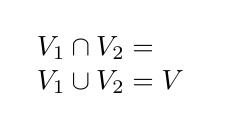
\begin{tikzpicture}[baseline={(A.base)}]
		\node [text width=2cm] (A) at (0,0) {$V_1 \cap V_2 = \varnothing$\\
			$V_1 \cup V_2 = V$};
	\end{tikzpicture}
\end{definition}

Смежными могут быть только вершины из разных долей графа.

\begin{center}
\begin{tikzpicture}
	\graph[nodes={draw, circle}] {
		subgraph I_nm [V={1, 2, 3}, W={4, 5}];
		
		1 -- { 4, 5};
		2 -- { 4, 5};
		3 -- { 5 }
	};

    \node[anchor=west] at (2, -0.5) {
        \begin{minipage}{4cm}
        \begin{align*}
            V &= \{1, 2, 3, 4, 5\} \\
            V_1 &= \{1, 2, 3\} \\
            V_2 &= \{4, 5\}
        \end{align*}
        \end{minipage}
    };
\end{tikzpicture}
\end{center}

\begin{definition}
    \textit{Полный двудольный граф} -- каждая вершина одной доли соединяется с другой.
    $K_{t_1, k_2}$, где ${t_1, k_2}$ -- количество вершин в долях графа.
\end{definition}

\begin{center}
\begin{tikzpicture}
	\graph[nodes={draw, circle}] {
		subgraph I_nm [V={1, 2, 3}, W={4, 5, 6}];
		
		1 -- { 4, 5, 6};
		2 -- { 4, 5, 6};
		3 -- { 4, 5, 6}
	};

    \node[anchor=west] at (2, -0.5) {
        \begin{minipage}{4cm}
        \begin{align*}
            K_{3,3}\\
            V &= \{1, 2, 3, 4, 5, 6\} \\
            V_1 &= \{1, 2, 3\} \\
            V_2 &= \{4, 5, 6\}
        \end{align*}
        \end{minipage}
    };
\end{tikzpicture}
\end{center}

В полном двудольном графе содержится $t_1 \cdot t_2$ ребер.